\documentclass[12pt]{article}
\usepackage{algos-tasks}

\begin{document}
\task[latex]{Getting Started with \LaTeX}

\LaTeX\ (pronounced ``\emph{lay}-tek'' or ``\emph{lah}-tek'') is a markup language that is commonly used to produce academic and technical writing. Typesetting in \LaTeX\ is quite different to word processors such as Microsoft Word, as the WYSIWYG (what you see is what you get) principle doesn't apply; instead, the document is a plain text file and is machine-interpreted into a form that is more human readable. Much like HTML files are rendered by a browser, \LaTeX\ files (with the extension \texttt{.tex}) are \emph{compiled} by an \emph{engine}.

One key outcome of this course is to familiarise yourself with the basics of \LaTeX. This exercise will help new students get started.

\subsection*{Why \LaTeX?}

\begin{itemize}
\item It's free to use.
\item The \texttt{.tex} file format is just plain text, so your documents don't rely on any proprietary software and can easily be worked on across different platforms.
\item Both the source code and the compiled document have very small file sizes.
\item It allows you to create very complex equations and graphics, as well as all the other document elements provided by a word processor.
\item It supports referencing within the document and to a bibliography with minimal effort (particularly useful for a thesis).
\item It separates content from presentation, so you can easily change the appearance of an existing document.
\item It is highly customisable, allowing you extensive control over how your document appears.
\item It is versatile, allowing you to write scientific articles, books, resum\'{e}s, slides, and more.
\item It is highly extensible, with a huge number of free additional packages to help you make just about anything you want.
\end{itemize}

\TeX\ was originally designed in 1978 by Donald Knuth; he was unsatisfied with the typesetting of the second volume of \textit{The Art of Computer Programming}, so he decided to design a better typesetting system himself!

\TeX\ has since had many extensions. By far the most widely used system is \LaTeX, designed in 1984 by Leslie Lamport, which adds many useful macros to base \TeX\ in order to make it easier to use.

\subsection*{Workflow}

We highly recommend that you use \href{https://www.overleaf.com/sso-login}{Overleaf}. You can register for a free professional account using your UNSW student email at the link above. Overleaf allows you to edit, compile and display your documents within a browser (and download them in PDF\footnote{\TeX\ was first designed for high-quality \emph{printing}, so the traditional compilation was $\texttt{.tex} \xrightarrow{\texttt{latex}} \texttt{.dvi} \xrightarrow{\texttt{dvips}} \texttt{.ps}$, but for \emph{viewing} documents, we simply use PDF.} format), and manage large projects. It also supports syncing with various cloud storage providers and version control systems.

To work on your local machine, you'll need a few more tools. We \emph{do not} recommend this workflow, but in case you really want to do this (e.g. for working offline):
\begin{itemize}
    \item You will need to install a TeX distribution. We recommend \href{https://tug.org/texlive/}{TeX Live} (or the Mac version, \href{https://tug.org/mactex}{MacTeX}), but \href{https://miktex.org}{MiKTeX} is a popular alternative.
    \item You'll also need a program to edit the source code.
    \begin{itemize}
        \item If you use a `basic' editor such as Vim or Emacs, you can compile your documents from the command line using \texttt{pdflatex}.
        \item If you use a more powerful editor such as Sublime Text or VS Code, you can compile your documents after selecting the appropriate build settings.
        \item There are also specialised editors such as TeXstudio, TeXworks, TeXShop and LyX, but we find that it's best to use software that you're already familiar with.
    \end{itemize}
    \item Finally, you'll need a PDF reader.
    \begin{itemize}
        \item Sublime Text users may wish to use \href{https://www.sumatrapdfreader.org/free-pdf-reader}{Sumatra PDF} on Windows or \href{https://skim-app.sourceforge.io/}{Skim} on Mac to support integrations such as inverse search.
    \end{itemize}
\end{itemize}

\subsection*{Hello, World!}

\subsubsection*{Your first \LaTeX\ document}

In almost every future written task, you can simply edit the stub provided in the Task Resources folder. This task however involves starting new files, as we're building up very simple documents.

Start with an empty file named \texttt{hello.tex}, and input the following.

\begin{lstlisting}
\documentclass{article}
\begin{document}
Hello, World! This is my first document using LaTeX.
\end{document}
\end{lstlisting}

\textbf{Warning:} Don't copy and paste from the PDF, as this will add extraneous spaces and newlines. You should instead copy and paste from the source code of the task sheet (\texttt{1.02 Hello, World!.tex}), or retype the code.

The section before \verb|\begin{document}| is called the \emph{preamble}, and it contains configuration options for the document. Here, we've chosen an \texttt{article} type document, without altering any settings (yet).

The remainder of the document is called the \emph{body}, and it contains the content of the document. For now, we've only included plain text, but we'll add more structure and formatting later on.

For now, build a PDF from your source code, and admire your first \LaTeX\ document.

\subsubsection*{Control sequences}

You may have noticed that throughout this task sheet, we have stylised the name of the language as \LaTeX. This will be our first example of a \emph{control sequence}; a backslash followed by a sequence of letters, which signifies a command.

Let's now edit the ``Hello, World!'' document. Place a backslash before the `L' in the final word, and recompile.

\begin{lstlisting} 
\documentclass{article}
\begin{document}
Hello, World! This is my first document using \LaTeX.
\end{document}
\end{lstlisting}

One of the most common compilation errors is ``Undefined control sequence'', which is reported when you use a control sequence that is invalid, i.e. one that is not defined in the base language or any packages you've included, usually because you have mistyped the control sequence. Note that control sequences are case-sensitive.

\subsubsection*{An aside about spacing}

Whitespace in \LaTeX\ is different to other typesetting systems. Whitespace in a \texttt{.tex} file is more \emph{semantic} than literal. Placing multiple spaces or a single line break in running text is equivalent to a single space.

\begin{lstlisting}
\documentclass{article}
\begin{document}
Hello,   World!
This is my first document using \LaTeX.
\end{document}
\end{lstlisting}

A double line break starts a new paragraph.

\begin{lstlisting}
\documentclass{article}
\begin{document}
Hello, World! This here is a very very very very long sentence which should ideally be more than one line in the PDF, but conveys no useful information.

This is my first document using \LaTeX. This is yet another very very very very long sentence for no reason than to make the default indentation settings apparent.
\end{document}
\end{lstlisting}

New paragraphs are indented on the first line by default.\footnote{See \href{https://www.overleaf.com/learn/latex/Paragraphs\_and\_new\_lines\#Paragraph\_indentation}{here} for how to change this, if you want.}

One case to watch out for: whitespace characters are not letters, so they can also mark the end of a control sequence instead of producing actual whitespace.

\begin{lstlisting}
\documentclass{article}
\begin{document}
Hello, World! This is my first \LaTeX document.
\end{document}
\end{lstlisting}

When compiled, no space will appear between the words ``\LaTeX'' and ``document''. We can either manually insert the space (using backslash-space: \verb|\LaTeX\ document|), or insert an empty group (using braces enclosing nothing to terminate the control sequence: \verb|\LaTeX{} document|).

\begin{lstlisting}
\documentclass{article}
\begin{document}
Hello, World! This is my first \LaTeX\ document.
\end{document}
\end{lstlisting}

\underline{Aside:} How might you typeset a backslash?

\subsubsection*{More on control sequences}

\verb|\LaTeX| is a very simple control sequence; it produces a constant output. The real power of control sequences comes from their ability to take arguments. Let's use italics to draw attention to the fact that this is our very first document.

\begin{lstlisting}
\documentclass{article}
\begin{document}
Hello, World! This is my \textit{first} \LaTeX\ document.
\end{document}
\end{lstlisting}

Everything within the braces is acted upon by the \verb|\textit| control sequence. We could also achieve the same effect using \verb|\emph|, which designates text to be emphasised in a way that is suitable for the context.

\begin{lstlisting}
\documentclass{article}
\begin{document}
Hello, World! This is my \emph{first} \LaTeX\ document.
\end{document}
\end{lstlisting}

We can nest control sequences, for example, to re-emphasise just what a big accomplishment it is to use \LaTeX\ for the first time.

\begin{lstlisting}
\documentclass{article}
\begin{document}
Hello, World! \emph{This is my \emph{first} \LaTeX\ document.}
\end{document}
\end{lstlisting}

What stands out within italicised text? Upright text!

You can also use control sequences to make text bold (\verb|\textbf|), underlined (\verb|\underline|) and more, which each take one argument as above.

However, some control sequences take two or more arguments. To make text a different colour, we'll use the \verb|\textcolor| control sequence, which is defined in the \texttt{xcolor} package. We'll first include that package in the preamble, and now we can use the commands defined there in the body.

\begin{lstlisting}
\documentclass{article}
\usepackage{xcolor}
\begin{document}
Hello, World! This is my \textcolor{red}{first} \LaTeX\ document.
\end{document}
\end{lstlisting}

\subsubsection*{Environments}

Some effects, particularly those which are larger in scope or significance, are defined using \emph{environments}. An environment is enclosed by \verb|\begin| and \verb|\end|. You have already seen one environment: \texttt{document} processes its contents as the body of the document.

\begin{lstlisting}
\documentclass{article}
\usepackage{xcolor}
\begin{document}
Hello, World! This is my \textcolor{red}{first} \LaTeX\ document.
\begin{center}
I can centre-align text using an environment!
\end{center}
\end{document}
\end{lstlisting}

We will see many important environments in later tasks, allowing us to make tables, insert graphics, draw our own graphics and much more.

\subsubsection*{Comments}

As with any other language, readability is important. It can be useful to include comments for portions of the document that are not to be typeset. The percent character `\%' denotes the beginning of an inline comment: the rest of that line will not affect the document.

\begin{lstlisting}
\documentclass{article}
\usepackage{xcolor} % pretty colours

\begin{document}
This is my \textcolor{red}{first} \LaTeX\ document. % yay!
\end{document}
\end{lstlisting}

Block comments are not a feature of the base language. However, the \texttt{verbatim} package provides a \texttt{comment} environment for this purpose.

\begin{lstlisting}
\documentclass{article}
\usepackage{xcolor} % pretty colours
\usepackage{verbatim}

\begin{document}
This is my \textcolor{red}{first} \LaTeX\ document.
\begin{comment}
TODO:
- add a title
- talk about future learning
\end{comment}
\end{document}
\end{lstlisting}

\underline{Aside:} how would you typeset a percentage symbol?

\subsubsection*{Document class features}

This text is nice, but it's rather small. The default font size is 10 point; let's increase it to 12. We can do this by providing an  argument to the document class. Some packages can also be included with optional arguments.

\begin{lstlisting}
\documentclass[12pt]{article}
\usepackage{xcolor}

\begin{document}
Hello, World! This is my \textcolor{red}{first} \LaTeX\ document.
\end{document}
\end{lstlisting}

Now, let's add a title to our document. The \texttt{article} document class allows us to define certain special variables in the preamble and then generate the title from them in the body.

\begin{lstlisting}
\documentclass[12pt]{article} % larger font
\usepackage{xcolor} % pretty colours

\title{Hello, World!}
\author{Your name here}
\date{Term X, 20YY}

\begin{document}
\maketitle
This is my \textcolor{colour}{first} \LaTeX\ document. I am \emph{very} excited to learn more features!
\end{document}
\end{lstlisting}

If the \verb|\date| control sequence is omitted from the preamble, then the system date will be used. You can provide an empty string as the argument to \verb|\date| if you want to leave out the date completely.

\subsubsection*{Lists}

We'd like to be able to make ordered and unordered lists, again in much the same way as the \texttt{<ol>} and \texttt{<ul>} tags in HTML, or numbered and bulleted lists in a word processor. \LaTeX\ achieves this using the \texttt{enumerate} and \texttt{itemize} environments respectively.

\begin{lstlisting}
\documentclass[12pt]{article} % larger font
\usepackage{xcolor} % pretty colours

\title{Hello, World!}
\author{Your name here}
\date{Term X, 20YY}

\begin{document}
\maketitle
This is my \textcolor{colour}{first} \LaTeX\ document. I am \emph{very} excited to learn more features!

Some animals I like are:
\begin{enumerate}
    \item my favourite animal,
    \item my second favourite animal, and
    \item my third favourite animal.
\end{enumerate}

Some of the books I've read include:
\begin{itemize}
    \item this book,
    \item that book, and
    \item that other book.
\end{itemize}
\end{document}
\end{lstlisting}

Note that \texttt{algos-tasks.sty} reconfigures the default numbering style from 1., 2., \dots to (a), (b), \dots. This style file is included in the solution stubs in the Task Resources, and you can use this styling in future tasks to set out your answers to each part.

\bigskip

\begin{question}
Copy the above snippet to \texttt{hello.tex}, then edit it with your name, the current term, your \href{https://www.overleaf.com/learn/latex/Using\_colors\_in\_LaTeX\#Named\_colors\_provided\_by\_the\_xcolor\_package}{favourite colour} and some animals and books.

\textbf{Reminder:} Don't copy and paste from the PDF, as this will add extraneous spaces and newlines. You should instead copy and paste from the source code of the task sheet (\texttt{1.02 Hello, World!.tex}), or retype the code.
\end{question}

\begin{rubric}
You should submit both the compiled PDF and the source code from the final example, with your name and the current term, and a colour of your choice.
\end{rubric}
\newpage
\subsection*{Document structure}

A \LaTeX\ document consists of two main parts; the \emph{preamble} and the \emph{body}.

\subsubsection*{Preamble}

The preamble contains information about how the document is to be configured.

The preamble begins by specifying a \emph{document class}, which is the type of document you want to produce. Some common examples include \texttt{article}, \texttt{book}, \texttt{letter}, \texttt{beamer} (for presentations) and \texttt{standalone} (for graphics). The format is \verb|\documentclass[options]{class}|.

Next, we include packages. These are the equivalent of libraries or headers in programming languages such as C, adding commands and functionalities that are not conveniently available in the base language. We will commonly include packages such as \texttt{amsmath} and \texttt{amssymb} (for mathematical symbols), \texttt{xcolor} (for colours), \texttt{listings} (for code formatting) and \texttt{hyperref} (for links), but there are thousands of packages on \href{https://ctan.org/pkg}{CTAN}. Packages can also be included with optional arguments.

We can also specify custom commands and macros, which will be discussed in a later task.

We can even include custom packages. In the \LaTeX\ templates for tasks in this course, you will see that the preamble always includes \verb|\usepackage{algos-tasks}|, which is a style (\texttt{.sty}) file containing various packages and macros that we use to typeset the tasks (and you might also find convenient in your responses).

\subsubsection*{Body}

In the body of the document, \LaTeX\ is always in one of three modes.
\begin{itemize}
    \item We won't discuss LR mode.
    \item Paragraph mode is the default, used for processing ordinary text.
    \item Math mode is used for equations, and has two submodes:
    \begin{itemize}
        \item \emph{inline} math mode is used for equations in running text, and
        \item \emph{display} math mode is used for equations on their own line.
    \end{itemize}
\end{itemize}

Inline math mode is delimited by either \verb|\(...\)| or \verb|$...$|, and display math mode is delimited by either \verb|\[...\]| or \verb|$$...$$|.

\underline{Aside:} How might you typeset a dollar sign?

Various mathematical symbols are typeset using control sequences, some of which can only be used in math mode.

\begin{lstlisting}
\documentclass[12pt]{article}
\usepackage{amsmath} % for maths
\title{Typesetting Mathematics}
\author{Your name here}

\begin{document}
\maketitle
The area of a circle is given by $A = \pi r^2$.

The quadratic formula states that the solutions to \(ax^2 + bx + c = 0\) are \[ x = \frac{-b \pm \sqrt{b^2-4ac}}{2a}. \]
\end{document}
\end{lstlisting}

It is often desirable to write a sequence of equations with alignment. For this, we'll use the \texttt{align*} environment\footnote{The unstarred version assigns an equation number, which we will only rarely need.} from the \texttt{amsmath} package. The ampersand `\texttt{\&}' is the alignment marker, and `\texttt{\textbackslash\textbackslash}' marks a new line.

\begin{lstlisting}
\documentclass[12pt]{article}
\usepackage{amsmath}
\title{Typesetting Mathematics}
\author{Your name here}

\begin{document}
\maketitle
The area of a circle is given by $A = \pi r^2$.

The quadratic formula states that the solutions to \(ax^2 + bx + c = 0\) are \[ x = \frac{-b \pm \sqrt{b^2-4ac}}{2a}. \]

For example, if $a = 2$, $b = -5$ and $c = 3$, then we have
\begin{align*}
x &= \frac{-(-5) \pm \sqrt{(-5)^2 - 4(2)(3)}}{2(2)}\\
&= \frac{5 \pm \sqrt{25-24}}{4}\\
&= \frac{5 \pm 1}{4}\\
&= \frac{3}{2} \text{ or } 1.
\end{align*}
\end{document}
\end{lstlisting}

Note the use of \verb|\text| to typeset the word ``or'' in plain text, rather than in the same style as the variable name $x$, and the explicit spacing around this word.

\subsubsection*{Sigma Notation}

When describing algorithms, we often use compact sigma notation to describe repeated operations. For example, the operation
\begin{verbatim}
    sum = 0
    for i = 1 to n:
        sum = sum + A[i]
\end{verbatim}

would be written as $\displaystyle \sum_{i=1}^n A[i]$. In \LaTeX, this is written as
\begin{lstlisting}
\documentclass[12pt]{article}
\usepackage{amsmath} % for maths
\title{Typesetting Mathematics}
\author{Your name here}
\begin{document}
\maketitle
The following sigma notation represents a for loop that sums all the elements of an array $A$ of length $n$.
\[\sum_{i=1}^{n} A[i].\]
\end{document}
\end{lstlisting}

The \verb|\sum| command takes two arguments, \verb|lower| and \verb|upper| each enclosed in \verb|{...}| that define the lower and upper bound for the summation's range. However, where the elements are not ordered (i.e. a set), we should omit the \verb|upper| argument. For example,  \[ \sum_{e \in E} \operatorname{weight}(e) \] denotes the sum of all the edge weights in a graph (all edges $e \in E$).

Other tips you might want to be wary of: 
\begin{itemize}
    \item When quoting, be wary of orienting your inverted commas correctly. Using two inverted commas (\verb|'|) before and after a quote will output two inverted commas in the same direction. You should use a backtick (\verb|`|) to open a quote, and a regular inverted comma to close the quote.
    \item It's often good to have a cheat sheet ready for commonly used control structures. There are many available online, and it might be worth writing your own as you go along. If you're unsure what command gives a particular symbol, \href{https://detexify.kirelabs.org/classify.html}{Detexify} is an helpful tool available online.
    \begin{itemize}
        \item It's often worth asking staff about certain norms; say, usage of the \verb|\left| and \verb|\right| operators, and not using the asterisk for multiplication.
    \end{itemize}
\end{itemize}


\newpage

\begin{question}
For this question, we want to practice using the \verb|\sum| command.
Copy the above snippet to \texttt{math.tex} and add the answers to the questions to \texttt{math.tex} in the \verb|enumerate| environment by using the \verb|\enumerate| command.
\begin{enumerate}
\item We want to write the expression 

\begin{center}
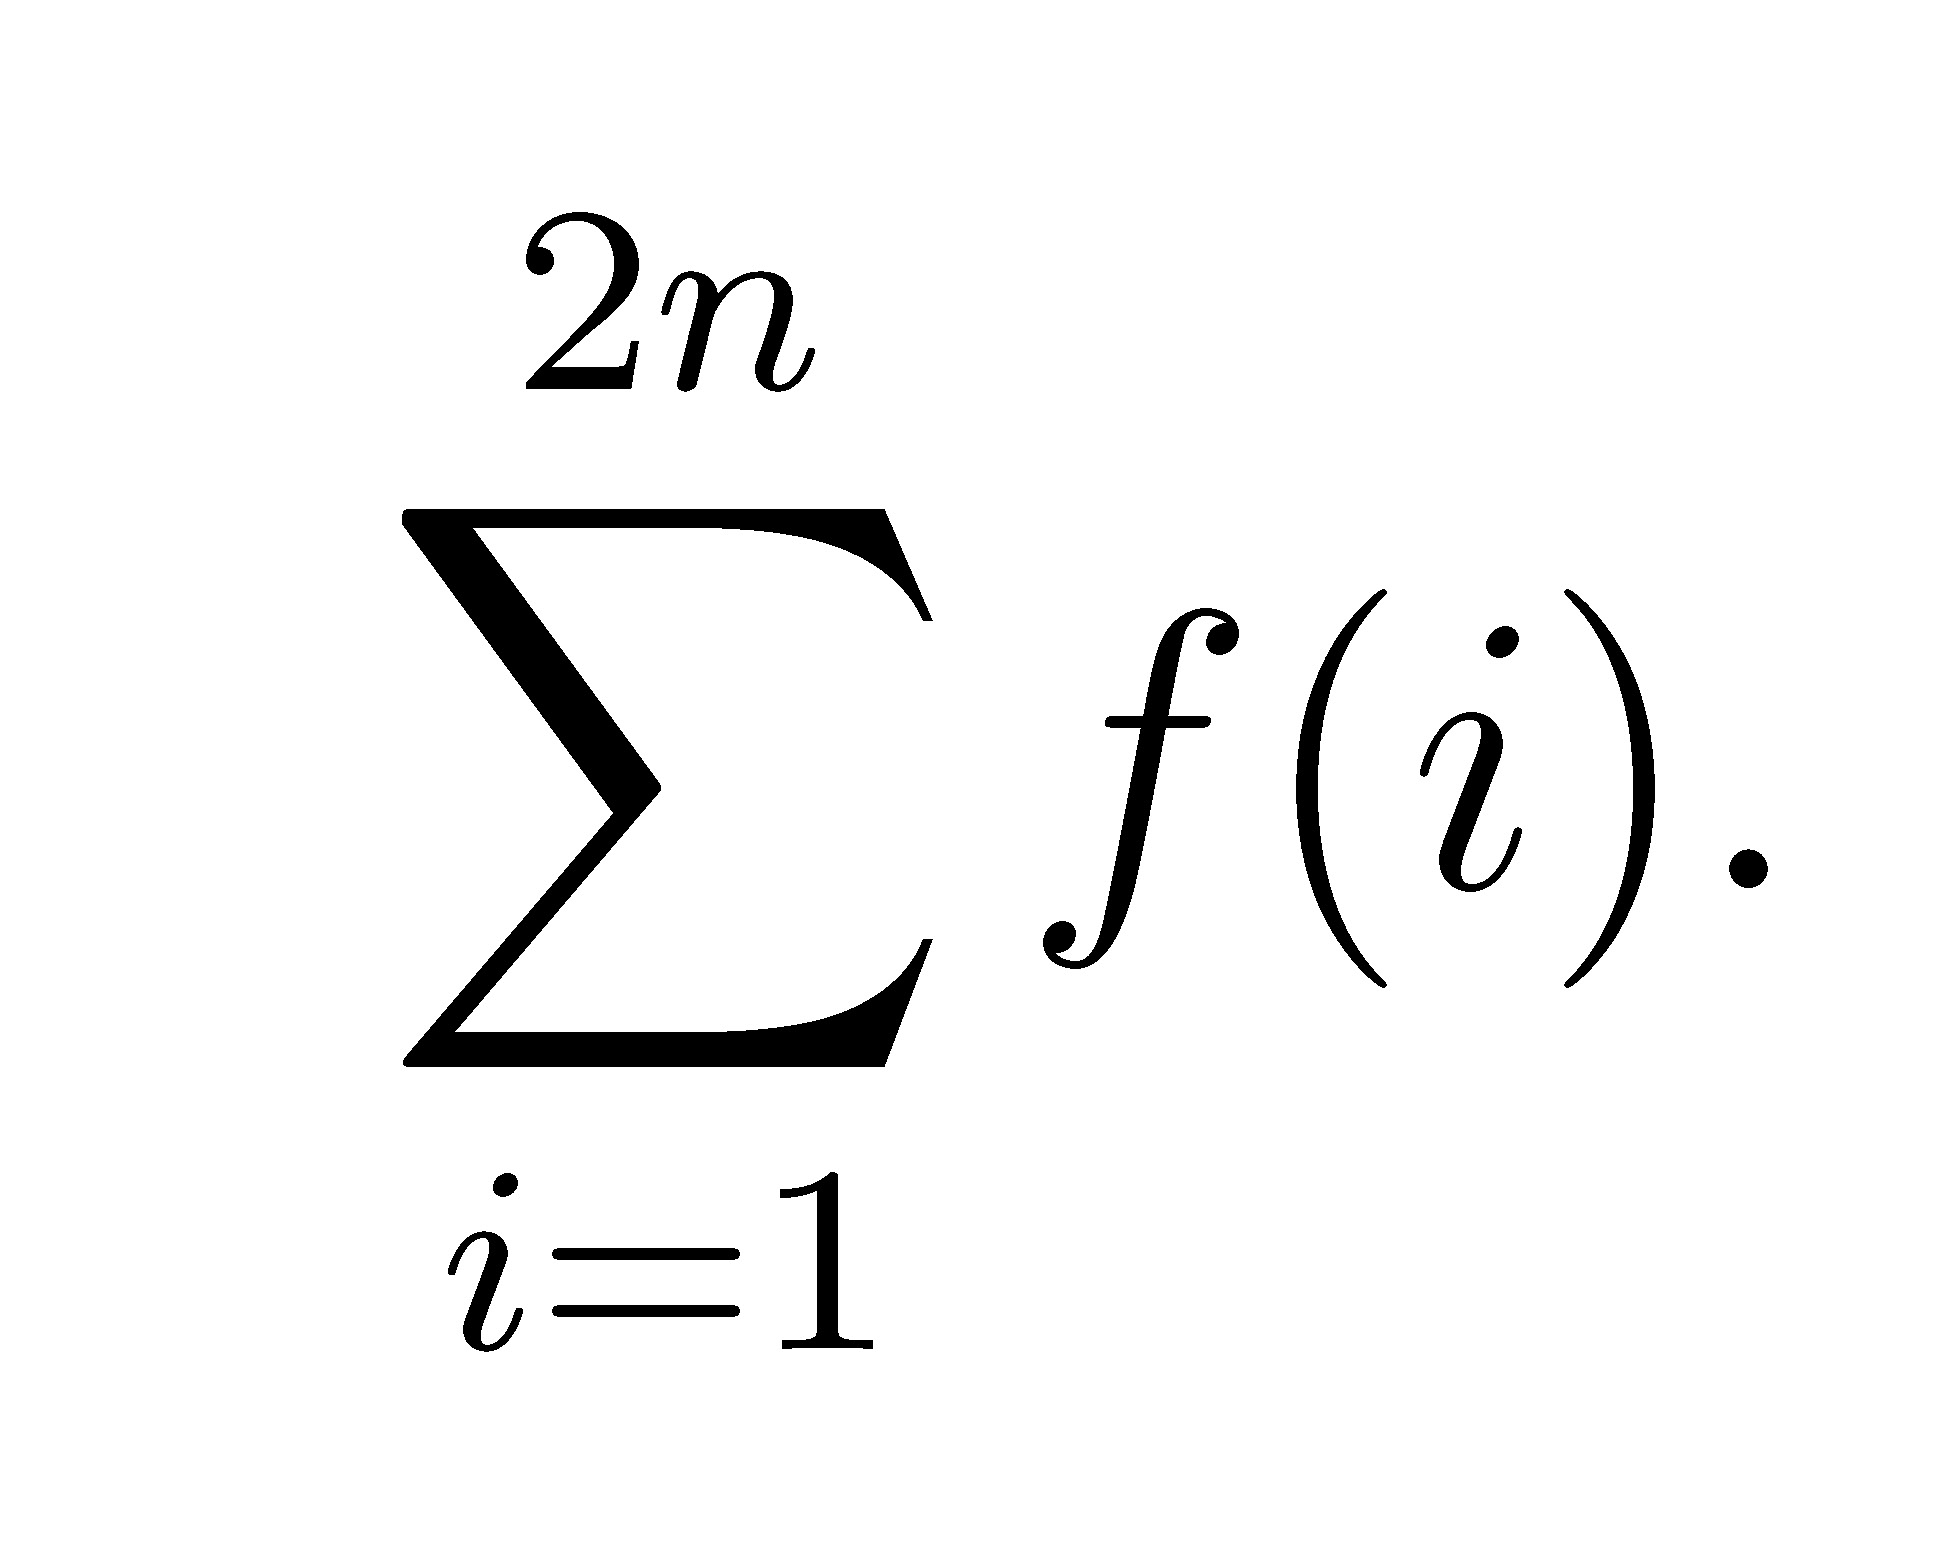
\includegraphics{eqn.jpg}
\end{center}
    We wrote the following \LaTeX\ code:
    \begin{center}
    \verb|\sum_i=1^2n f(i)|
    \end{center}
    What output does this produce? Identify and correct the errors in the code.
    \item Using sigma notation, write an expression for the total absolute difference between each pair of adjacent elements in an array $A$ of length $n$. For example, given the array $A = [1, 4, 2, 3]$, the total absolute difference is $\abs{1-4} + \abs{4-2} + \abs{2-3} = 6$.

    \textbf{Note:} \verb|\abs{...}| is not a control sequence defined in base \LaTeX\ or the maths packages, but rather a macro that we've defined in \texttt{algos-tasks.sty}. You can instead use \verb|\abs*{...}| for bars which scale with the height of the enclosed content.
\end{enumerate}

\textbf{Reminder:} Don't copy and paste from the PDF, as this will add extraneous spaces and newlines. You should instead copy and paste from the source code of the task sheet (\texttt{1.02 Hello, World!.tex}), or retype the code.
\end{question}


\begin{rubric}
    You should submit both the compiled PDF and the source code for this question, and answer all the subparts. Detailed instructions for submission are available as comments in \texttt{hello.tex} and \texttt{math.tex} in the Task Resources folder.
\end{rubric}

\end{document}